\chapter{Theoretical framework}
\label{chp:theory}

\section{Quark parton model and DIS}
\label{sec:basicDIS}
By the time of 1960s, people have discovered a large range of hadrons 
in various experiments and reactions following certain conservation laws
which may convert one type of hadron to another type. Analysis performed on these 
conservation laws and the properties of these hadrons indicates that
there exists some common substructure that forms all the hadronic objects.


Suggested by Gell-Mann and Zweig in 1964, a group of point-like particles named
as quarks can be used to describe this fundamental substructures that build up
the hadron hierarchy. For instance, in the naive picture, a proton is made up of
two ``up" quarks and one ``down" quark. These quarks are supposed to be fermions
with fractional charge following the SU(3) symmetry. Due to the color confinement
feature of the strong force, there is no isolated fractional electric charge ever
seen in a detector. However, although it is impossible to directly detect these
elementary constituents, one can still obtain the their information with the
structureless lepton probes bombarding hadrons similar to the strategies of the
``Rutherford-prime" experiment.

This type of study was firstly performed at the Stanford Linear Accelerator
Center (SLAC) experiment with 20 GeV electron beams bouncing off proton
target~\cite{Panofsky:1966gq}. The electron proton scattering process performed
at this experiment can be illustrated by Fig.~\ref{fig:DIS_kinematics} with the
notation of \( e(k)+p(P) \rightarrow e(\kp) + X, \) where $X$ represents any
hadronic final systems allowed by conservation laws. The process is mediated by
a virtual vector boson, with 4-momentum given by $q=k-\kp$.

\begin{figure}
\centering
\includegraphics[width=0.5\textwidth]{plots/chpt2/DIS_kinematics.png} 
\caption[Schematic diagram of a DIS process] {
Schematic diagram of DIS scattering via virtual photon exchange.}
\label{fig:DIS_kinematics}
\end{figure}

The selection of Lorentz invariant variables describing the process in
Fig.~\ref{fig:DIS_kinematics} is only a matter of convention, but the following
set of the kinematics variables is commonly used:
\begin{enumerate}
\item The squared center-of-mass (CM) energy
\begin{equation}
	s = (k+P)^{2}.
\end{equation}

\item The magnitude of momentum transfer mediated by the virtual boson
\begin{equation}
Q^{2} = -q^{2} = -(k-\kp)^{2},
\end{equation}
at intermediate $Q^{2}$ only photon exchange needs to be considered.

\item Bjorken scaling variable
\begin{equation}
x_{Bj} = \frac{Q^{2}}{2P\cdot q},
\end{equation}
which can be interpreted as momentum fraction of
struck quark taken from the incoming nucleon in the quark parton model.

\item The inelasticity
\begin{equation}
y = \frac{P\cdot q}{ P\cdot k},
\end{equation}
giving fraction of the electron energy transfered to
the hadronic system.

\item The energy current transfered from lepton in the target rest frame
\begin{equation}
\nu = \frac{P\cdot q}{ M_{p} }.
\end{equation}

\item The invariant mass of the final state hadronic system
\begin{equation}
W^{2} = (P+q)^{2}.
\end{equation}

\end{enumerate}

If we denote the proton mass by $M_{p}$, the introduced variables are related by
$Q^{2}=(s-M^{2}_{p})x_{Bj}y$, $\nu = ys/(2M_{p})$ and
$W^{2}=M^{2}_{p}+Q^{2}\frac{1-x_{Bj}}{x_{Bj}}$. It can be found in these
equations that only two variables are independent at fixed center-of-mass
energy. If not specified, all the plots in this thesis follow the beam direction
convention: the hadron beam goes to $+z$ and such to positive rapidities are
often referred to as ``forward'' direction, while the electron beam goes to $-z$
and the electron beam going direction is often termed as ``backward'' direction
towards to negative rapidities.



With large momentum transfer \qsq, we are allowed to resolve smaller objects
having transverse momenta less than $Q$ and localized within a transverse
area $\sim 1/Q^{2}$.
The regime of $Q^{2}\gg M^{2}_{p}$ and $W^{2}\gg M^{2}_{p}$ is often referred
to as the DIS regime. Therefore, the proton mass term can be ignored in the relations
for $Q^{2}$ and $W^{2}$ in DIS collisions.

If $Q^{2}$ is much smaller than the mass of $Z^{0}$ boson (neglecting electroweak effects), the DIS process
can be approximately described with the assumption of a one-photon exchange. Then,
the double differential DIS cross section can be expressed as:
\begin{equation}
\frac{d^{2}\sigma}{dx_{Bj}dQ^{2}}=\frac{4\pi\alpha^{2}}{Q^{4}}[y^{2}F_{1}(x_{Bj},Q^{2})+(1-y)\frac{F_{2}(x_{Bj},Q^{2})}{x_{Bj}}].
\end{equation}
In this formula, $\alpha$ represents the fine structure constant. $F_{1}$ and
$F_{2}$ are commonly parameterized frame invariant structure functions for
protons. $F_{1}$ describes the pure magnetic part of the interaction while $F_{2}$
corresponds to the sum over the electromagnetic contribution. A longitudinal structure function can
be defined through $F_{L}(x_{Bj},Q^{2})=F_{2}(x_{Bj},Q^{2})-2x_{Bj}F_{1}(x_{Bj},Q^{2})$,
which reforms the double differential cross section to:
\begin{equation}
\frac{d^{2}\sigma}{dxdQ^{2}}=\frac{2\pi\alpha^{2}}{x_{Bj}Q^{4}}[YF_{2}(x_{Bj},Q^{2})-y^{2}F_{L}(x_{Bj},Q^{2})],
\end{equation}
where $Y=1+(1-y)^{2}$. $F_{2}$ and $F_{L}$ can be practically measured in
inclusive scattering. The \ep\ scattering experiment at SLAC showed that the
structure functions had no dependence on $Q^{2}$, a phenomena called Bjorken scaling 
(for example, see Fig.~\ref{fig:F2_pdg} at $x_{Bj}\sim0.25$).

\begin{figure}
\centering
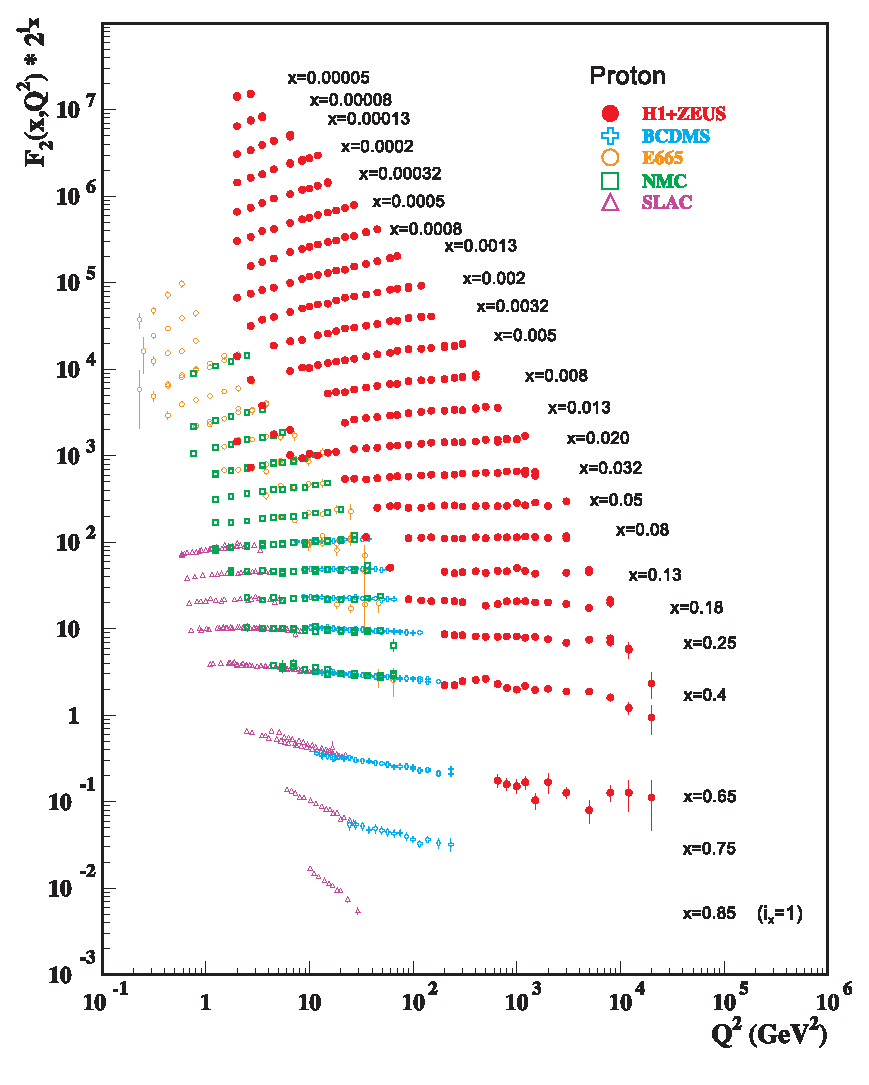
\includegraphics[width=0.85\textwidth]{plots/chpt2/f2collider_logf2.eps}
\caption[Combined proton structure function F2 distribution from different experiments] {
The combined proton structure function $F_{2}$ data from HERA and fixed target experiments at different $x_{Bj}$ (denoted by $x$ in this plot) as a function of $Q^{2}$. The plot is from the PDG tables ~\cite{Beringer:1900zz}.}
\label{fig:F2_pdg}
\end{figure}

The quark parton model was firstly introduced by Feynman to interpret the
scaling behavior observed in the SLAC data. The basic assumption of this model
is to represent the electron proton scattering as an incoherent sum of
scatterings on some individual point-like constituents within the proton called
partons. It is postulated that the partons binded in the proton are effectively
free. To satisfy this requirement, the quark parton model must be defined in the
infinite momentum frame with $P\rightarrow\infty$. In this model, without the
dependence on $Q^{2}$, the structure function $F_{2}$ can be interpreted as
follows
\begin{equation}
F_{2}(x_{Bj})=\sum_{i=q,\bar{q}}e^{2}_{i}x_{Bj}f_{i}(x_{Bj}),
\label{eqn:F2_QPM}
\end{equation}
which sums over partons with charge $e_{i}$. $f_{i}(x_{Bj})$ is the probability
of finding a parton $i$ carrying a fraction $x_{Bj}$ of the proton's momentum.
The $f_{i}(x_{Bj})$ is known as the parton distribution function (PDF). The PDF
is assumed to be universal and can be used for different target particles with
various combinations in a wide range of physics processes. 

Although the parton model is shown to be successful in describing a lot
experimental data especially in DIS collisions, a number of paradoxes remain.
For instance, there is a clear breaking of the Bjorken scaling in the $F_{2}$
data at large and small x which cannot be incorporated in the quark parton
model. The study in momentum sum rule suggests that the momentum carried by
quarks and antiquarks do not add up to the total momentum of protons. This fact
implies that there are other important components in the proton except for
quarks and antiquarks. Besides, no individual quarks ever observed in a free
state. These paradoxes shed some light on the development of QCD as the theory
of strong force. We will see how the puzzles in the simple quark parton model
are solved with the elements of QCD theory derived in the next section.




\section{Quantum chromodynamics} \label{sec:QCD}
QCD is the theory of strong interaction~\cite{Politzer:1974fr}. A gauge
boson, called gluon, is introduced to this framework as the mediator of strong
force. The theory postulates the color degree of freedom with three possible
values, red, green and blue, and correspondingly the anti-colors. The gluons
couple to all particles carrying color charges. While the gluons themselves
carry color charges, it is possible to have gluon self-interactions. The crucial
outcome is that QCD provides the feature of color confinement at large distances
keeping color charges binded in the hadrons and asymptotic freedom allowing to
have essentially free quark interactions at short distances. The strength of
strong interaction is described by the QCD coupling $\alpha_{s}$. This coupling
is predicted to be small in high-energy collisions, which makes it possible to
use perturbation theory in these occasions~\cite{Lipatov:1974qm}.


\subsection{Asymptotic freedom and confinement}
Asymptotic freedom is a feature of QCD that causes forces between partons weaker
as energy increases or distance decreases. This feature arises in a similar way
to the consideration of screening for the electric charge in the quantum
electrodynamics (QED)~\cite{Feynman:1950ir, Gockeler:1997dn}. The vacuum in QED
is assumed to be consisted of virtual electron-positron pair fluctuations in
field theory. In the vicinity of an electric charge, the polarization of these
virtual fluctuations in the vacuum becomes important and partially cancels out
the net charge sitting at the center. The same thing happens in QCD, with the
vacuum being quark-antiquark pairs plus the virtual gluons. Since gluons carry
charge themselves, the vacuum state of gluons in the medium has paramagnetism.
The effect of virtual gluons in the vacuum is to augment the center color charge
instead of screen it, sometimes called antiscreening. So the antiscreening
effect of surrounding virtual gluons at small separations diminishes, the color
interaction becomes feeble under these circumstances (small distance or high
energy). This feature can be mathematically expressed in the running of QCD
coupling $\alpha_{s}$.

\begin{figure}
\centering
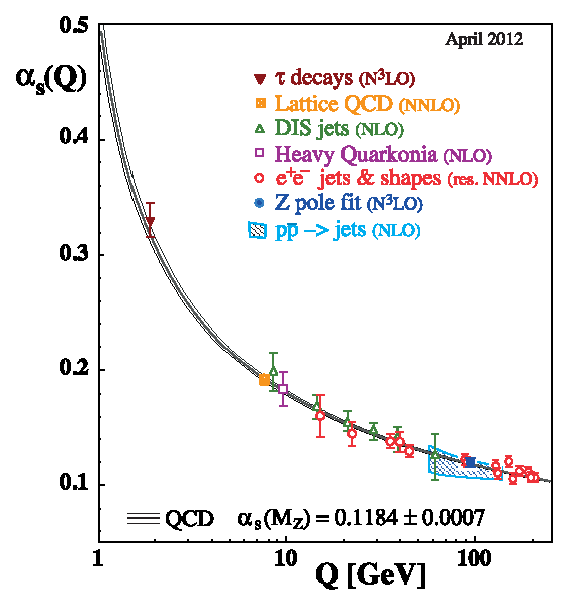
\includegraphics[width=0.6\textwidth]{plots/chpt2/asq.eps}
\caption[Measurements of running coupling $\alpha_{s}$ versus $Q$] {
Measurements of $\alpha_s$ versus $Q$. The plot is from the PDG tables ~\cite{Beringer:1900zz}.}
\label{fig:alpha_s}
\end{figure}

The derivation of asymptotic freedom in QCD needs to calculate the beta-function
describing $\alpha_{s}$ with the renormalization group equation (RGE). In the
one-loop approximation, the running of QCD coupling $\alpha_{s}(Q^{2})$ is
generally expressed by~\cite{Collins:1987pm}
\begin{equation}
\alpha_{s}(Q^{2})=\frac{4\pi N_{c}}{(11N_{c}-2N_{f})\ln(Q^{2}/\Lambda^{2}_{QCD})},
\label{eqn:alphas}
\end{equation}
where $N_{c}$ is the number of color degrees of freedom. $N_{f}$ shows the
number of active quark flavors. $\Lambda_{QCD}$ specifies the energy scale at
which the perturbative coupling becomes infinite. As is shown in
Fig.~\ref{fig:alpha_s}, the coupling $\alpha_{s}(Q^{2})$ becomes essentially
small at large $Q^{2}$.

Formally, Eq.~\ref{eqn:alphas} predicts the divergence of coupling
$\alpha_{s}(Q^{2})$ and the breakdown perturbative QCD theory when $Q^{2}$
approaches $\Lambda^{2}_{QCD}$. But this equation can not be trusted for
$Q\lesssim 1$ GeV, since it is derived from the perturbation theory. Although it
is still debatable about fate of $\alpha_{s}$ for $Q\sim\Lambda_{QCD}$, various
non-perturbative approaches suggest that QCD coupling should be relatively large
(roughly at a value around one). As a consequence, the quarks and gluons should
be confined in the colorless hadrons due to the growth of coupling at low scales
and can not escape as free particles.


\subsection{Factorization}
The microscopic picture of high-energy scattering process involves fluctuated
parton configuration of hadrons in the initial state (see
Fig.~\ref{fig:hadron_config} for an example). We have to deal with the
constantly emitted and absorbed virtual fluctuations in the QCD vacuum. 

\begin{figure}
\centering
\includegraphics[width=0.5\textwidth]{plots/chpt2/hadron_initial_state.png}
\caption[proton initial state parton configurations] {
Schematic view of proton initial partonic fluctuations. The plot is from Ref.~\cite{Skands:2012ts}. }
\label{fig:hadron_config}
\end{figure}

If we revisit the DIS process illustrated in Fig.~\ref{fig:DIS_kinematics}, we
will find that the virtual fluctuations are confined in the proton with a life
time $\sim 1/\Lambda_{QCD}$. On the other hand, the electromagnetic probe
interacts with the proton at a much shorter time scale $1/Q \ll
1/\Lambda_{QCD}$. During the interaction, the microscopic configuration inside
the proton is almost frozen and can be viewed as a superposition of free,
independent partons (as assumed in Feynman's quark parton model). A snapshot of
the proton inner structure is taken by the virtual photon probe. The scattering
involving a hard probe allowing us to apply the purterbation method like this is
usually referred to as the hard scattering process. Practically, the hard probe
must have a scale $Q^{2}>1 \mathrm{GeV}^{2}$. It is then possible to factorize
the DIS cross section into the product of a process-independent non-perturbative
PDF and a perturbatively calculable hard partonic cross
section~\cite{Sterman:1995fz}.

It is very common to separate the perturbative and non-perturbative parts of the
cross section by applying the collinear factorization scheme, in which the
struck parton is approximately collinear with the proton beam momentum. The DIS
cross section can be expressed in collinear factorization as follows
\begin{equation}
\sigma(ep\rightarrow eX')=\sum_{i} \int^{1}_{0}\frac{dx}{x}f_{i}(x,\mu^{2})\hat{\sigma_{i}}.
\label{eqn:coll_factor}
\end{equation}
$f_{i}$ is the same PDF as explained in Eq.~\ref{eqn:F2_QPM} with $\mu^{2}$
being the factorization scale and $\hat{\sigma_{i}}$ is the hard partonic cross
section. It is convenient to choose the factorization scale to be the exchanged
photon virtuality $\mu=Q$ in DIS collisions. $x$ is the momentum fraction of the
parton involved in the hard interaction. It is equal to $x_{Bj}$ if we focus on
the LO DIS process. For higher oder DIS process, $x$ is larger than $x_{Bj}$ as
shown in the forthcoming discussions. The PDF $f_{i}$ is not priori calculable
and must be constrained by fits to experimental data~\cite{Aaron:2009aa}, while
the partonic cross section $\hat{\sigma_{i}}$ is calculable within the
perturbation theory.


\section{DIS in QCD framework}\label{sec:DISinQCD}
In perturbative QCD (pQCD) framework, for a given physical quantity, the cross
section is calculated by expanding amplitudes in perturbation series of
$\alpha_{s}$. The leading order (LO) DIS diagram is of zeroth order of
$\alpha_{s}$ corresponding to Fig.~\ref{fig:LODIS}, while the next to leading
order (NLO) tree level DIS processes at $\mathcal{O}(\alpha_{s}^{1})$ are shown
in Fig.~\ref{fig:PGF} and Fig.~\ref{fig:QCDC} usually named as Photon-Gluon
Fusion (PGF) process and QCD Compton (QCDC) process, respectively. For the DIS process at LO,
the PGF and QCDC processes are considered as the real corrections, while the
virtual corrections displayed in Fig.~\ref{fig:VirtCorr} also need to be
included. After renormalization, both real and virtual processes will contribute to collinear and soft singularities. It is proven~\cite{Kinoshita:1962ur,Lee:1964is} that for suitable observables, these singularities from real and virtual correction will cancel leaving finite higher order remainders when added together. In the
collinear factorization scheme, these uncanceled collinear singularities with a
scale up to $Q^{2}$ will be absorbed into the scale dependent PDF $f_{i}(x,Q^{2})$. The
scale dependence contributing to the DIS cross section
can be described within the parton evolution scheme. It is expected that the
parton evolution leads to the violation of Bjorken scaling in $F_{2}(x,Q^{2})$.

\begin{figure*}
	\begin{center}
	\subfigure[]{
		\centering
		\includegraphics[width=0.25\textwidth]{plots/chpt6/feynman/LODIS.eps}
		\label{fig:LODIS}
	}
	\quad
	\subfigure[]{
		\centering
		\includegraphics[width=0.25\textwidth]{plots/chpt6/feynman/PGF.eps}
		\label{fig:PGF}
	}
	\quad
	\subfigure[]{
		\centering
		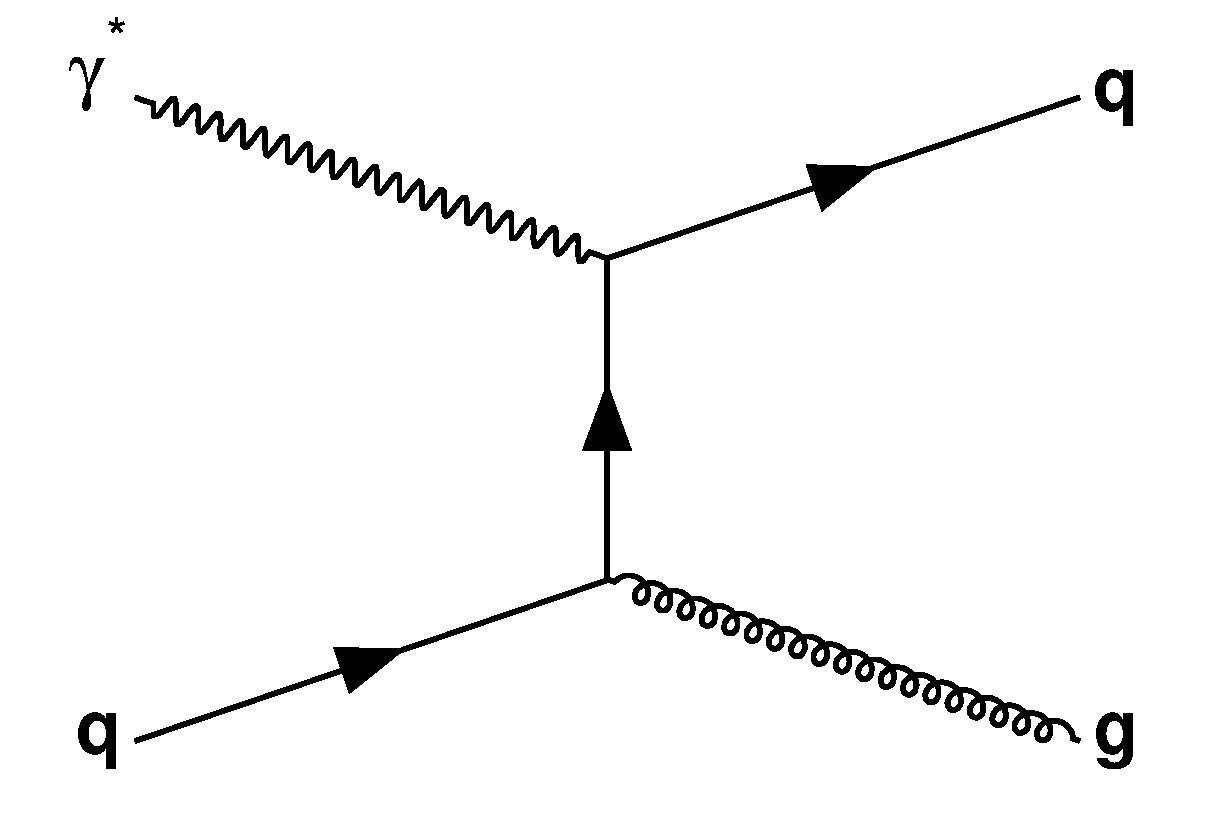
\includegraphics[width=0.25\textwidth]{plots/chpt6/feynman/QCDC.eps}
		\label{fig:QCDC}
	}
	\caption[LO and NLO DIS feynman diagrams]{Feynman diagrams for the hard processes 
	based on point-like photons: (a) $\mathcal{O}(\alpha^{0}_{s}) $ LO DIS, (b) 
	Photon-Gluon Fusion (PGF) and (c) QCD Compton scattering (QCDC).}
	\label{fig:DISgraph}
	\end{center}
\end{figure*}


\begin{figure}
\centering
\includegraphics[width=0.8\textwidth]{plots/chpt2/virtual_correction.png}
\caption[virtual corrections] {
Illustration of higher oder virtual corrections to LO DIS. }
\label{fig:VirtCorr}
\end{figure}


\subsection{DGLAP evolution equations}
As is mentioned above, the size and shape of PDF $f_{i}(x,Q^{2})$ is not
calculable in pQCD framework but the scale dependence in $Q^{2}$ for PDF can be
derived from the evolution equations. The $Q^{2}$ evolution of PDF is described
through the Dokshitzer-Gribov-Lipatov-Altarelli-Parisi (DGLAP)
formalism~\cite{Dokshitzer:1977sg,Gribov:1972ri,Altarelli:1977zs}. The essence
of the DGLAP approach is the perturbation treatment of splitting functions. The
splitting functions $P_{ij}(z)$ describe the probability of a
mother parton $i$ splitting into a daughter partons $j$ with momentum fraction
$z$ by emitting a parton $k$ with fraction $1-z$ of the mother parton's
momentum, as demonstrated in Fig.~\ref{fig:split_fun}.

\begin{figure}
\centering
\includegraphics[width=0.5\textwidth]{plots/chpt2/split_fun.png}
\caption[Splitting functions] {
Illustration of diagrams corresponding to the splitting functions. The plot is from Ref.~\cite{Belov:2013oda}. }
\label{fig:split_fun}
\end{figure}

The LO expression for splitting function is given by


\begin{align}
& P_{qq}(z)=\frac{4}{3}[\frac{1+z^{2}}{(1-z)_{+}}+\frac{3}{2}\delta(1-z)], \\
& P_{qg}(z)=\frac{1}{2}[z^{2}+(1-z)^{2}], \\
& P_{gq}(z)=\frac{4}{3}[\frac{1+(1-z)^{2}}{z}], \\
& P_{gg}(z)=6[\frac{1-z}{z}+\frac{z}{(1-z)_{+}}+z(1-z)]+[\frac{33-2N_{f}}{6}\delta(1-z)],
\end{align}
in which $[f(z)]_{+}=f(z)-\delta(1-z)\int^{1}_{0}f(t)dt$.
The DGLAP equations give a rigorous formalism for calculating the changes of PDF
as $Q^{2}$ varies, the PDF shape and size at an initial scale $Q^{2}_{0}$ has to
come either from non-perturbative methods or parameterization in $x$ with
parameters determined by QCD fits to data.

With the DGLAP evolution scheme, the scaling violation effect of $F_{2}$ can be
explained in the QCD framework. As shown in Fig.~\ref{fig:F2_pdg}, the violation
to Bjorken scaling is observed for large $x$ ($x>0.4$) and small $x$ ($x<0.02$)
region. For the large $x$ part, valence quarks dominate the distribution. Since
the struck quark is taking a large fraction of the proton momentum, it is likely
to radiate a gluon as $q\rightarrow qg$. With increasing $Q^{2}$, more gluon
radiations like this will be resolved and the contribution to $F_{2}$ will be
shifted to smaller $x$ value, which is why we see a drop in $F_{2}$ versus
$Q^{2}$. On the other hand, gluons or sea quarks dominate at small $x$. Higher
$Q^{2}$ identifies the process of a gluon splitting into a pair of sea quarks
$g\rightarrow q\bar{q}$, which explains the rise of $F_{2}$ as $Q^{2}$
increases.

\subsection{Evolution at small $x$}
The DGLAP equation in the lowest order resums the leading terms of
$\alpha_{s}\ln(Q^{2})$, while the sub-leading terms involve powers of
$\alpha_{s}\ln(1/x)$. In regions where $x$ is small, the DGLAP approximation is
not valid ($\alpha_{s}\ln(1/x)$ becomes more important than
$\alpha_{s}\ln(Q^{2})$) and a different approach, the so-called
Balitsky-Fadin-Kuraev-Lipatov (BFKL) evolution equation~\cite{Balitsky:1978ic}
has been developed. The BFKL equation is a linear evolution equation and it
governs the evolution of the gluon distribution with respect to $x$ at fixed
$Q^{2}$. The corresponding factorization formula is known as
$k_{T}$-factorization, involving the unintegrated parton distribution function
(uPDF). Then, the \ep\ cross section can be written as
\begin{equation}
\sigma(ep\rightarrow eX')=\sum_{i} \int\frac{dx}{x}dk_{T}^{2}\mathcal{F}_{i}(x,k_{T})\hat{\sigma_{i}}.
\end{equation}
Compared to Eq.~\ref{eqn:coll_factor}, the uPDF can be related to integrated PDF
as \[f_{i}(x,Q^{2})\simeq \int^{Q^{2}}_{0}dk_{T}^{2}\mathcal{F}_{i}(x,k_{T}).\]
At the small $x$, the gluon density grows much faster than the quark density and
is the major component for the proton wave function. Therefore, for the small
$x$ considerations, we shall focus on the gluons alone. The solution of BFKL
equation exhibits a rapid increase of gluon density as $x$ gets smaller.
However, the gluon density cannot grow arbitrarily large, since this would
violate the unitarity limit for forward scattering amplitudes or the Froissart
bound for total cross sections at very high energies. Recent experimental data
at rather small $x$ have provided us some intriguing evidence for the existence
of a novel QCD regime, namely the saturation regime, which cannot be fully
described by linear QCD evolution
approaches~\cite{Stasto:2000er,Armesto:2004ud,Gelis:2010nm}. In the next
chapter, we will have more comprehensive discussions about the physics in
saturation regime.





